\documentclass{article}
\usepackage{amsmath} 
\usepackage{graphicx} 
\usepackage{authblk}
\usepackage{url}
\usepackage{hyperref}
\usepackage{multirow}
\usepackage{amssymb}
\usepackage{subcaption}
\usepackage[linesnumbered,boxed]{algorithm2e}

\topmargin 0.0cm
\oddsidemargin 0.2cm
\textwidth 16cm 
\textheight 21cm
\footskip 1.0cm

\title{Numerical Method for Ordinary differential equations and Its Application in Physics}
\author[1]{Mengzhi Chen}
\author[1]{Tong Li}
\affil[1]{Department of Physics and Astronomy, Michigan State University}
\date{}

\begin{document}
	\maketitle
	\begin{abstract}\label{abstract}
Tong
	\end{abstract}

\section{Introduction}\label{intro} 
	Tong
	
\section{Examples of ordinary differential problems in physics}\label{physcis_problem}
	
	\subsection{The Earth-Sun system}\label{earthsun}
	The Earth-Sun system is a two-body system governs by the attractive gravitational force between them
\begin{equation}
	\vec{F}_G = \frac{GM_{\mathrm{S}}M_{\mathrm{E}}\hat{r}}{r^2},
\end{equation}
where G is the gravitational constant; 
$M_{\mathrm{S}}$ and $M_{\mathrm{E}}$ are mass of the Sun and the Earth; $\vec{r}$ is the displacement between them.

Given the fact the Sun is about $10^6$ heavier than the Earth, we can safely keep the Sun as the center of mass (C.M.) in this problem. 
With a proper coordinate setup, the orbit of the Earth is co-planer in $xy$-plane. 
Using Newton's second law we get the following first-order ordinary differential equations (ODEs) for the Earth

\begin{equation}
	\label{earthsunodes}
	\left\{  
             \begin{array}{lr}  
             	\frac{dx}{dt} = v_x \\
				\frac{dx}{dt} = v_x \\
            	\frac{dv_x}{dt} = -\frac{GM_{\mathrm{S}}x}{r^3} \\
				\frac{dv_y}{dt} = -\frac{GM_{\mathrm{S}}y}{r^3}.
			\end{array}  
	\right.	
\end{equation}

By solving above equations, we can obtain the informations about the Earth's orbit we need.

	
	\subsection{Many body problem}\label{quantumdot}
	In the above Sec. \ref{earthsun}, we simplify the calculation of the orbit of the Earth by taking into account only it's interaction with the Sun. 
This simplification is reasonable as the Sun is much heavier than other planets in the solar system. 

However, if we want to go a step further to get a more precise description of the Earth's orbit. 
We have to include distortions from other seven planets as well as the Pluto.
We should also abandon our previous static Sun approximation but using the real center of mass of the solar system.
Until now, we have a new set of ODEs for the Earth

\begin{equation}
	\left\{  
             \begin{array}{lr}  
             	\frac{dx}{dt} = v_x \\
				\frac{dy}{dt} = v_y \\
            	\frac{dv_x}{dt} = \sum\limits_{i=1}^{n}-\frac{GM_{\mathrm{i}}x_i}{r_i^3} \\
				\frac{dv_y}{dt} = \sum\limits_{i=1}^{n}-\frac{GM_{\mathrm{i}}y_i}{r_i^3},
			\end{array}  
	\right. 	
\end{equation}
where $i$ runs over all other celestial bodies except the Earth itself. 
Besides the Earth, we have similar sets of ODEs for every celestial body.

By solving these coupled ODEs, we can obtain a full description for the solar system.

	
\section{Numerical methods}\label{method}
  
	\subsection{Euler forward method}\label{euler}
	Suppose a first-order ordinary differential equation

\begin{equation}
	\frac{dx}{dt} = f(x,t);\ t\in[t_0,t_1]
\end{equation}
with a initial value $x_0$ at time $t_0$. 

In order to solve this problem, we first discretize the region $ [t_0,t_1]$ into N subintervals with a step $h$, so we get the relation

\begin{equation}
	h=\frac{t-t_0}{N}.
\end{equation}
Then, We have discretized $x_i=x(t_i=t_0+ih)$ where $i$ is a integer between 0 and $N$.

Using Taylor expansion, we get 

\begin{equation}
	\label{eulerexpan}
	x_{i+1} = x_i + \frac{dx_i}{dt}h + \frac{d^2x_i}{dt^2}h^2 + O(h^3),
\end{equation}
where i goes from 0 to $N-1$.
The Euler's forward method truncates at the second term of the above equation.
Thus, Eq. \ref{eulerexpan} becomes

\begin{equation}
	\begin{aligned}
		x_{i+1} & = x_i + \frac{dx_i}{dt}h + O(h^2) \\ 
				& = x_i + f(x_i,t_i)h + O(h^2).
	\end{aligned}
\end{equation}
We can see it's a one-step method with a local error $O(h^2)$.

Getting back to the Earth-Sun system, we can formulate Eq. \ref{earthsunodes} to

\begin{equation}
	\left\{  
             \begin{array}{lr}  
             	x_{i+1} = x_i + v_x^{i}h \\
				y_{i+1} = y_i + v_y^{i}h \\
             	v_x^{i+1} = v_x^{i} - \frac{4\pi^2x_i}{r_i^3}h\\
             	v_y^{i+1} = v_y^{i} - \frac{4\pi^2y_i}{r_i^3}h.
			\end{array}  
	\right.	
\end{equation} 
in unit of AU for length, year (yr) for time and $M_{\mathrm{S}}$ for mass. 
We will keep using this unit system in our report and calculations. 
Starting from some initial conditions, we can simply solve out time evolution of the Earth iteratively. 
Our implementation of this method with a  circular orbit initial conditions is shown in Algorithm \ref{alg::euler}. 

\begin{algorithm}[tb]
	\caption{The Euler's forward method for the Earth-Sun system. It initials from a circular orbit.}
	\label{alg::euler}
	\KwIn{$x_0=1$, $y_0=0$, $v_{x}^0=0$, $v_{y}^0=2\pi$, $M_{\mathrm{E}}$, $M_{\mathrm{S}}$, $G$ }
	\KwOut{$\vec{x}$=($x_0$,$x_1$,...,$x_N$), $\vec{y}$, $\vec{v}_x$, $\vec{v}_y$, $\vec{E}_k$, $\vec{E}_p$, $\vec{E}$, $\vec{L}_z$} 
	$r$ = sqrt($x_0^2$+$y_0^2$)\;
	// $i$ is deferent time points $t_i=t_0+ih$\;
    \For{$i=1;i<=N;i++$}
    { $x_{i} = x_{i-1} + v_x^{{i-1}}h$;
    $y_{i} = y_{i-1} + v_y^{{i-1}}h$\;
    $v_x^{i} = v_x^{i-1} - \frac{4\pi^2x_{i-1}}{r_{i-1}^3}h$;
    $v_y^{i} = v_y^{i-1} - \frac{4\pi^2y_{i-1}}{r_{i-1}^3}h$\;
    $r$ = sqrt($x_i^2$+$y_i^2$)\;
    // Kinetic energy $E_k$, Potential energy $E_k$, Total energy $E$, Angular momentum in $\hat{z}$ $L_z$\;
    $E_k^i$ = 0.5$M_{\mathrm{E}}$($(v_x^{i})^2$+$(v_y^{i})^2$);
    $E_p^i$ = $-\frac{GM_{\mathrm{E}}M_{\mathrm{S}}}{r}$\;
    $E^i$ = $E_p^i$ + $E_k^i$;
    $L_z^i$ = $M_{\mathrm{E}}(x_iv_y^{i}-y_iv_x^{i})$\;
    }
	return $\vec{x}$, $\vec{y}$, $\vec{v}_x$, $\vec{v}_y$, $\vec{E}_k$, $\vec{E}_p$, $\vec{E}$, $\vec{L}_z$\;
\end{algorithm}

We can see that the Euler's forward method is easy to be realized.
 However, it has vital defects that it violates the energy conservation and time reversibility.
 The total energy increases with time in the Euler's forward method.
 That's why we need the Velocity-Verlet method to describe physical systems.

	
	\subsection{Velocity-Verlet method} \label{verlet}
	The velocity-Verlet method is widely used in molecular dynamics calculation as it overcomes these defects. It conserves energy with small round-off errors\cite{toxvaerd2012energy}.

Staring from the Taylor expansions under same discretization

\begin{equation}
	\begin{aligned}
		x_{i+1} = x_i + x_i^{(1)}h + x_i^{(2)}h^2 + O(h^3),\\
		v_x^{i+1} = v_x^{i} + v_x^{i(1)}h + v_x^{i(2)}h^2 + O(h^3),
	\end{aligned}
\end{equation}
with a initial value $x_0$ and $v_x^0$ at time $t_0$. We truncate at the third term and evaluate $v_x^{i(2)}h \approx v_x^{i+1(1)}-v_x^{i(1)}$. We can see that velocity-Verlet method is a two-step method with a local error $O(h^3)$

In the Earth-Sun system, with this method, we can formulate Eq. \ref{earthsunodes} to

\begin{equation}
	\left\{  
             \begin{array}{lr}  
             	x_{i+1} = x_i + v_x^{i}h - \frac{4\pi^2x_i}{r_i^3}\frac{h^2}{2} \\
				y_{i+1} = y_i + v_y^{i}h - \frac{4\pi^2y_i}{r_i^3}\frac{h^2}{2} \\
             	v_x^{i+1} = v_x^{i} - (\frac{4\pi^2x_i}{r_i^3}+\frac{4\pi^2x_{i+1}}{r_{i+1}^3})\frac{h}{2}\\
             	v_y^{i+1} = v_y^{i} - (\frac{4\pi^2y_i}{r_i^3}+\frac{4\pi^2y_{i+1}}{r_{i+1}^3})\frac{h}{2}.
			\end{array}  
	\right.	
\end{equation} 
We show our realization of the velocity-Verlet method in Algorithm \ref{alg::verlet}. Compared with the Euler forward method, we can see the calculations in this method is more complicated.

\begin{algorithm}[tb]
	\label{alg::verlet}
	\caption{The Velocity-Verlet method for the Earth-Sun system. It initials from a circular orbit.}
	\KwIn{$x_0=1$, $y_0=0$, $v_{x}^0=0$, $v_{y}^0=2\pi$, $M_{\mathrm{E}}$, $M_{\mathrm{S}}$, $G$ }
	\KwOut{$\vec{x}$=($x_0$,$x_1$,...,$x_N$), $\vec{y}$, $\vec{v}_x$, $\vec{v}_y$, $\vec{E}_k$, $\vec{E}_p$, $\vec{E}$, $\vec{L}_z$} 
	$r$ = sqrt($x_0^2$+$y_0^2$)\;
	$a_x^0$ = $\frac{4\pi^2x_{i-1}}{r_{i-1}^3}$;
    $a_y^0$ = $\frac{4\pi^2y_{i-1}}{r_{i-1}^3}$\;
	// $i$ is deferent time points $t_i=t_0+ih$\;
    \For{$i=1;i<=N;i++$}
    {$x_{i} = x_{i-1} + v_x^{i-1}h - \frac{a_x^0h^2}{2}$;
    $y_{i} = y_{i-1} + v_y^{i-1}h - \frac{a_y^0h^2}{2}$\;
    $r$ = sqrt($x_i^2$+$y_i^2$)\;
    $a_x^1$ = $\frac{4\pi^2x_{i}}{r_{i}^3}$;
    $a_y^1$ = $\frac{4\pi^2y_{i}}{r_{i}^3}$\;
    $v_x^{i} = v_x^{i-1} - \frac{(a_x^0+a_x^1)h}{2}h$;
    $v_y^{i} = v_y^{i-1} - \frac{(a_y^0+a_y^1)h}{2}h$\;
	$a_x^0$ = $a_x^1$;
    $a_y^0$ = $a_x^1$\;
    // Kinetic energy $E_k$, Potential energy $E_k$, Total energy $E$, Angular momentum in $\hat{z}$ $L_z$\;
    $E_k^i$ = 0.5$M_{\mathrm{E}}$($(v_x^{i})^2$+$(v_y^{i})^2$)\;
    $E_p^i$ = $-\frac{GM_{\mathrm{E}}}{r}$;
    $E^i$ = $E_p^i$ + $E_k^i$\;
    $L_z^i$ = $M_{\mathrm{E}}(x_iv_y^{i}-y_iv_x^{i})$\;
    }
	return $\vec{x}$, $\vec{y}$, $\vec{v}_x$, $\vec{v}_y$, $\vec{E}_k$, $\vec{E}_p$, $\vec{E}$, $\vec{L}_z$\;
\end{algorithm}

	
	\subsection{Object oriented code development}\label{obj}
	Tong
	
\section{Results and discussion}\label{results}

	\subsection{Comparison between two methods}
	To test the stability of Euler forward (Euler) and the velocity-Verlet (VV) method, we initialize the Earth-Sun system with a circular orbit as stated in Algorithms \ref{alg::euler,alg::verlet}.

We varies the step size $h$ starting from 0.02 yr to 0.001 yr.
The Earth's orbits calculated by these two methods for 10 years are show in Fig. \ref{fig::earth}. 
Globally speaking, we see orbits given by the Euler method expand in time.  
On the other hand, VV methods' orbits keep circular with some tiny fluctuation hardly seen in Fig. \ref{fig:earth500}.
It justifies the our statements in Sec. \ref{method} that the VV method conserves energy but the Euler method increase energy.

For a large step size in Fig. \ref{fig:earth500}, the Euler method is very unstable. Its orbit deviates from circle both in distance and shape apparently. 
As the step size becomes smaller, we can see that the Euler method becomes better; as the orbits expand slower and slower from \ref{fig:earth500} to Fig. \ref{fig:earth10000}.
 The trends we observed agree with the statement that the error in the Euler method goes down with decreasing $h$. We can hardly see differences between orbits yielded from the VV method, which indicates the it's stability.
 
\begin{figure}[tb]
	\begin{subfigure}[tb]{0.5\textwidth}
		\centering
		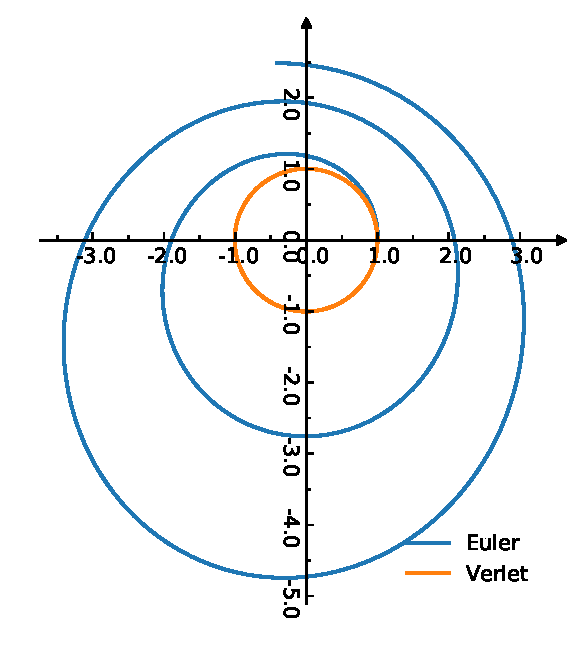
\includegraphics[width=0.7\textwidth]{Earth500.eps}
		\caption{$h = 0.02$yr}
		\label{fig:earth500}
	\end{subfigure}
~
	\begin{subfigure}[tb]{0.5\textwidth}
		\centering
		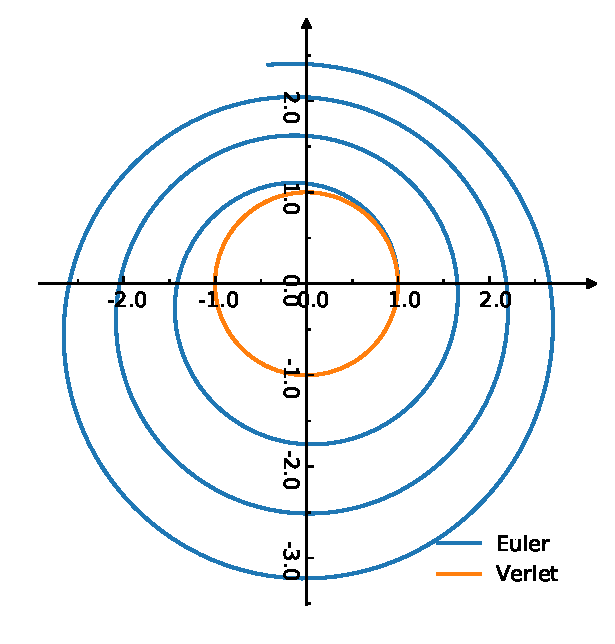
\includegraphics[width=0.7\textwidth]{Earth1000.eps}		\caption{$h = 0.01$year}
		\label{fig:earth1000}
	\end{subfigure}
~
	\begin{subfigure}[tb]{0.5\textwidth}
		\centering
		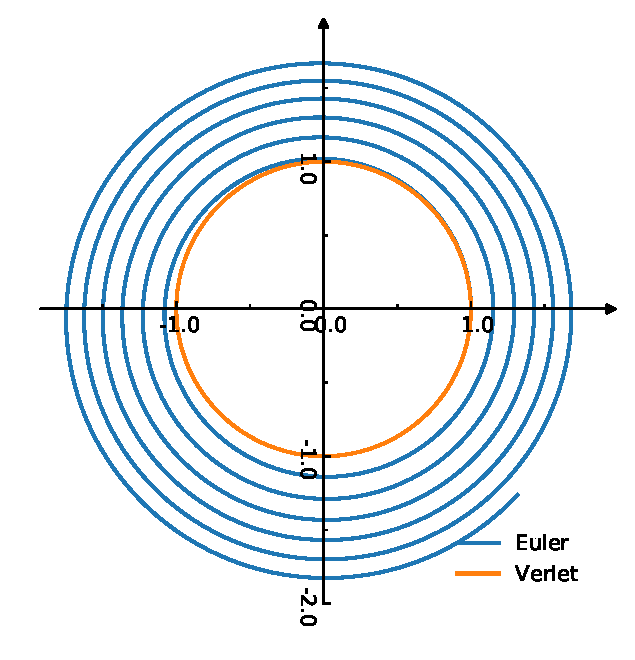
\includegraphics[width=0.7\textwidth]{Earth5000.eps}		\caption{$h = 0.002$year}
		\label{fig:earth5000}
	\end{subfigure}
~
	\begin{subfigure}[tb]{0.5\textwidth}
		\centering
		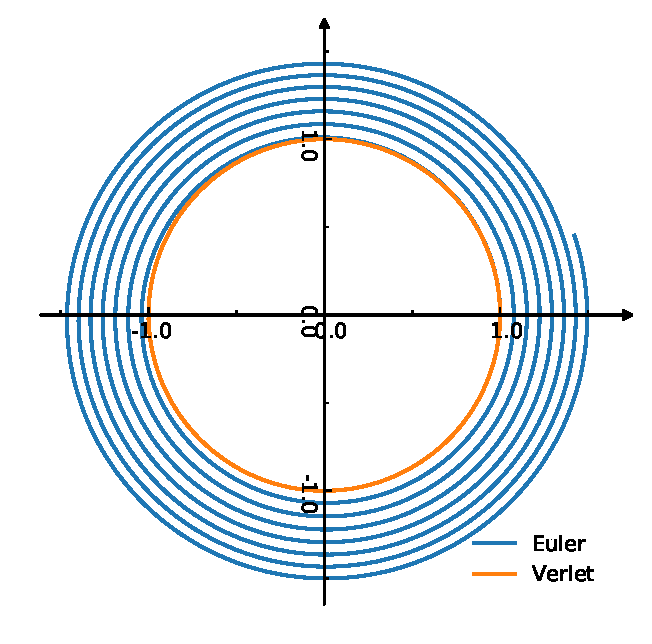
\includegraphics[width=0.7\textwidth]{Earth10000.eps}		\caption{$h = 0.001$year}
		\label{fig:earth10000}
	\end{subfigure}
	\caption{Comparison of different step size $h$ of two methods for 10 years. }
	\label{fig::earth}
\end{figure}

 For detailed check and performance comparison, we list distances, energies, angular momentums together with execution times for these two methods in Table \ref{tab::euler}\&\ref{tab::verlet} with precision up to $10^{-6}$.
 As conservation laws predicted by classical mechanics, physical quantities including kinetic, potential, total energies and angular momentum should be conserved in the Earth-Sun system. 
 From these two tables, we can see conservations in the VV method but not in the Euler method. Thus, we can conclude that the VV method is stable and the Euler method is not.
 
 Compared the execution time of two methods, we find the Euler method is faster. 
 Counting the FLOPS from these two algorithms, we find there is  about 30$N$ for the Euler method and 45$N$ for the VV method. It explains speed advantage of the Euler method.
 
\begin{table}[tb]
	\centering
	\caption{The Euler forward method: step size; kinetic energy; potential energy; total energy; angular momentum in z direction, distance from the Sum and execution time from left to the right.}
	\label{tab::euler}
	\begin{tabular}{ccccccc}
	\hline
	\hline
$h$          & $E_{kin}$        & $E_{pot}$         & $E_{tot}$          & $L_z$        & $r$         & execution time (ms)         \\
	\hline
2.000E-02 & 3.300E-05 & -4.700E-05 & -1.400E-05 & 3.500E-05 & 2.520E+00 & 2.500E-02 \\
1.000E-02 & 2.900E-05 & -4.900E-05 & -2.000E-05 & 3.200E-05 & 2.432E+00 & 5.000E-02 \\
2.000E-03 & 3.200E-05 & -6.500E-05 & -3.300E-05 & 2.500E-05 & 1.824E+00 & 9.400E-02 \\
1.000E-03 & 4.000E-05 & -7.900E-05 & -4.000E-05 & 2.300E-05 & 1.493E+00 & 1.680E-01\\
	\hline
	\hline
\end{tabular}
\end{table}

\begin{table}[tb]
	\centering
	\caption{The Velocity-Verlet method: step size; kinetic energy; potential energy; total energy; angular momentum in z direction, distance from the Sum and execution time from left to the right.}
	\label{tab::verlet}
	\begin{tabular}{ccccccc}
	\hline
	\hline
$h$          & $E_{kin}$        & $E_{pot}$         & $E_{tot}$          & $L_z$        & $r$         & execution time (ms)         \\
	\hline
2.000E-02 & 5.900E-05 & -1.180E-04 & -1.180E-04 & 1.900E-05 & 1.000014 & 2.600E-02 \\
1.000E-02 & 5.900E-05 & -1.180E-04 & -1.180E-04 & 1.900E-05 & 1.000E+00 & 5.600E-02 \\
2.000E-03 & 5.900E-05 & -1.180E-04 & -1.180E-04 & 1.900E-05 & 1.000E+00 & 1.840E-01 \\
1.000E-03 & 5.900E-05 & -1.180E-04 & -1.180E-04 & 1.900E-05 & 1.000E+00 & 3.350E-01\\
	\hline
	\hline
\end{tabular}
\end{table}

For physically meaningful, we will keep using the VV method in our further calculations.

	\subsection{Escape velocity against the Sun}
	MZ
	
	\subsection{Extension to whole solar system}
	Tong
	
	\subsection{The perihelion precession of Mercury}
	MZ
	
\section{Conclusions}\label{conclude}
Tong
	
	\section*{Acknowledgments}
	We are grateful for the sincere guidance from Prof. Morten Hjorth-Jensen. 
	
	\nocite{*} 
	\bibliographystyle{plain}
	\bibliography{proj3_ref}
\end{document}